%%
%%   Version 3.1 of 31 July 2018.
%%
\documentclass[aip,jcp,preprint,amsmath,amssymb,floatfix]{revtex4-1}
%\documentclass[aip,reprint]{revtex4-1}

\usepackage{graphicx}% Include figure files
\usepackage{dcolumn}% Align table columns on decimal point
\usepackage{bm}% bold math

% hyphenation
\usepackage{hyphenat}

% tables
\usepackage{multirow}
\usepackage{booktabs}

% mathematics
\usepackage{amsmath}
\usepackage{amsfonts}
\usepackage{amssymb}
\usepackage{amsbsy}
\usepackage{mathrsfs}
\usepackage{upgreek}

%---------------------------------------------------
% happy integral
\newcommand{\rint}[1]{\mbox{\Large $ \int\limits_{\mbox{\tiny  $#1$}}$}}
% SHORTCUTS
%\newcolumntype{,}{D{.}{,}{2}}
\newcommand{\citee}[1]{\ensuremath{\scriptsize^{\citenum{#1}}}}
\newcommand{\HRule}{\rule{\linewidth}{0.2mm}}
% Quantum notation
\newcommand{\bra}[1]{\ensuremath{\bigl\langle {#1} \bigl\lvert}}
\newcommand{\ket}[1]{\ensuremath{\bigr\rvert {#1} \bigr\rangle}}
\newcommand{\braket}[2]{\ensuremath{\bigl\langle {#1} \bigl\lvert {#2} \bigr\rangle}}
\newcommand{\tbraket}[3]{\ensuremath{\bigl\langle {#1} \bigl\lvert {#2} \bigl\lvert {#3} \bigr\rangle}}
% Math
\newcommand{\pd}{\ensuremath{\partial}}
\newcommand{\DR}{\ensuremath{{\rm d} {\bf r}}}
%\newcommand{\BM}[1]{\ensuremath{\mbox{\boldmath${#1}$}}}
\newcommand{\BM}[1]{\bm{#1}}
% Chemistry (formulas)
\newcommand{\ch}[2]{\ensuremath{\mathrm{#1}_{#2}}}
% Math 
\newcommand{\VEC}[1]{\ensuremath{\mathrm{\mathbf{#1}}}}
% vector nabla
\newcommand{\Nabla}{\ensuremath{ \BM{\nabla}}}
% derivative
\newcommand{\FDer}[3]{\ensuremath{
\bigg(
\frac{\partial #1}{\partial #2}
\bigg)_{#3}}}
% diagonal second derivative
\newcommand{\SDer}[3]{\ensuremath{
\biggl(
\frac{\partial^2 #1}{\partial #2^2}
\biggr)_{#3}}}
% off-diagonal second derivative
\newcommand{\SSDer}[4]{\ensuremath{
\biggl(
\frac{\partial^2 #1}{\partial #2 \partial #3}
\biggr)_{#4}}}
% derivatives without bound
% derivative
\newcommand{\fderiv}[2]{\ensuremath{
\frac{\partial #1}{\partial #2}}}
% diagonal second derivative
\newcommand{\sderiv}[2]{\ensuremath{
\frac{\partial^2 #1}{\partial #2^2}
}}
% off-diagonal second derivative
\newcommand{\sderivd}[3]{\ensuremath{
\frac{\partial^2 #1}{\partial #2 \partial #3}
}}
% derivatives for tables
\newcommand{\fderivm}[2]{\ensuremath{
{\partial #1}/{\partial #2}}}
% diagonal second derivative
\newcommand{\sderivm}[2]{\ensuremath{
{\partial^2 #1}/{\partial #2^2}
}}
% off-diagonal second derivative
\newcommand{\sderivdm}[3]{\ensuremath{
{\partial^2 #1}/{\partial #2 \partial #3}
}}
% ERIs and OEIs
\newcommand{\OEIc}[3]{\ensuremath{\left(#1 \lvert #2 \rvert #3 \right)}}
\newcommand{\ERIc}[4]{\ensuremath{\left(#1 #2 \vert #3 #4 \right)}}

% Partial density and potential
\newcommand{\PartPot}[4]{\ensuremath{\frac{#1 #2}{\lvert #3-#4 \rvert }}}

% trace operator
\DeclareMathOperator{\Tr}{Tr}

% EU logo
\newcommand*{\InlineImage}[1]{%
    \raisebox{-.02\baselineskip}{%
        \includegraphics[
        height=\baselineskip,
        width=\baselineskip,
        keepaspectratio,
        ]{#1}%
    }%
}

%\draft % marks overfull lines with a black rule on the right

\begin{document}

%\preprint{AIP/123-DMS}

\title{One-Particle Density Matrix Polarization Susceptibility Tensors}

\author{Bartosz B{\l}asiak}
\email[]{blasiak.bartosz@gmail.com}
\homepage[]{http://www.polonez.pwr.edu.pl}
\affiliation{Department of Physical and Quantum Chemistry, Faculty of Chemistry, 
Wroc{\l}aw University of Science and Technology, 
Wybrze{\.z}e Wyspia{\'n}kiego 27, Wroc{\l}aw 50-370, Poland}

\date{\today}

\begin{abstract}

The electric field\hyp{}induced change in the one\hyp{}electron density
has been expressed as a series of the one\hyp{}particle density matrix 
susceptibilities (DMS) interacting with the spatial distribution of electric field.
The analytic approximate expressions are derived at the Hartree\hyp{}Fock theory, 
which serves as a basis for construction of generalized model 
that is designed for an arbitrary form of wavefunction and any type of one\hyp{}particle density matrix.
It is shown that it is possible to accurately predict 
the changes in the one\hyp{}electron ground\hyp{}state density of water molecule 
in spatially uniform electric field, as well as in spatially non\hyp{}uniform 
electric field distribution generated by point charges. When both linear 
and quadratic terms with respect to the electric field are accounted for,
the electric field\hyp{}induced polarization energies, dipole moments 
and quadrupole moments are quantitatively described by the present theory 
in electric fields ranging from weak to very strong (0.001 -- 0.07 a.u.).
It is believed that the proposed model could open new routes in quantum chemistry 
for fast and efficient calculations of molecular properties in condensed phases.
\end{abstract}

\pacs{}% insert suggested PACS numbers in braces on next line

\maketitle %\maketitle must follow title, authors, abstract and \pacs

\section{\label{s:1}Introduction}

Molecular\hyp{}level exploration of condensed phase phenomena becomes increasingly unavoidable
as technology and medicine continue to develop. Unfortunately, the computational cost of accurate
electronic structure calculations grows extremely fast with the number of particles, greatly limiting
the use of the state\hyp{}of\hyp{}the\hyp{}art first\hyp{}principles theories when large and complex 
chemical systems such as solutions and biomolecules come into play.\cite{
Xu.Guidez.Bertoni.Gordon.JCP.2018,Tomasi.Mennucci.Cammi.ChemRev.2005}
Due to this reason, it has been of particular importance nowadays to develop bridging theoretical techniques 
that link extremely accurate but localized pieces of information with certain knowledge of an atomistic 
organization and intermolecular interaction on relatively large spatial scales, typically ranging beyond 
few nanometers. 

The development of hybrid methods such as quantum mechanical\hyp{}molecular mechanical (QM/MM) technique 
was a revolution in computational chemistry which allows insightful theoretical studies of quantum mechanical
effects in biological systems because costly quantum mechanical calculations can be combined with lower\hyp{}level 
and much less expensive classical dynamics.\cite{Warshel.Levitt.JMolBiol.1976,Senn.Thiel.Angew.2009}
Combination of accurate \emph{ab initio} methods with extensive experimental and semi\hyp{}empirical
refinings led to development of a wide variety of force fields,\cite{Demerdash.Yap.T-Head-Gordon.AnnuRevPhysChem.2014}
whereas sophisticated partitioning of Hamiltonian or electron density enabled numerous schemes for efficient fragmentation
within a QM level.\cite{Gordon.Fedorov.Pruitt.Slipchenko.ChemRev.2012}

However, even with the modern advances in computational chemistry, accurate description of phenomena due 
to complex heterogeneous molecular environments remains a challenge in the following areas: (i) describing 
the electronically excited states (electronic solvatochromism),\cite{Barbati.JACS.2014,
Szabla.Sponer.Jiri.Gora.JPCL.2015,Bednarska.Zalesny.Tian.Murugan.Agren.Bartkowiak.Molecules.2017,
Jedrzejewska.Grabarz.Bartkowiak.Osmialowski.SpectChimActA.2018} 
(ii) understanding the vibrational properties of molecules in ground and electronically excited states
(vibrational or vibronic solvatochromisms).\cite{Blasiak.Londergan.Webb.Cho.ACR.2017,
Xu.Blasiak.Cho.Layfield.Londergan.JPCL.2018,Lewis.Gruenke.Oliver.Ballottari.Bassi.Fleming.JPCL.2016} 
Interface between QM and MM levels is usually realized by electrostatic embedding and only rarely 
the Pauli exclusion principle and dispersion are additionally included.\cite{List.Olsen.Kongsted.PCCP.2016}
Unfortunately, it is quite difficult to efficiently treat the environment\hyp{}induced potential operator
due to complicated nature of intermolecular interactions that theoretically cannot be solely envisioned 
as a sum of separate contributions coming from electrostatic, dispersion and Pauli 
effects.\cite{Jeziorski.Moszynski.Szalewicz.ChemRev.1994} 
For example,
one of the most frequently used, efficient and reasonably accurate \emph{ab initio} fragmentation methods, 
the effective fragment potential (EFP) methods, are limited to the Hartree\hyp{}Fock 
(HF)\cite{Roothaan.RevModPhys.1951,Gordon.Smith.Xu.Slipchenko.AnnuRevPhysChem.2013} 
or density functional theory (DFT) levels\cite{Hohenberg.Kohn.PhysRev.1964,Kohn.Sham.PhysRev.1965,Nguyen.Pachter.Day.JCP.2014}.
While they can approximately describe the environment composed of molecules in their ground states,
they cannot be used for highly correlated wavefunctions such as electronically excited states. 
In such cases, the full QM method needs to be utilized on the excited state wavefunction, that is 
embedded within the EFP environment through the electrostatic or polarizable embedding.\cite{Ghosh.JPCA.2017}

Most of the efforts to theoretically treat extended molecular aggregates are rooted in energy\hyp{}based 
philosophy. However, in the past two decades there has been considerable interest in density\hyp{}based approaches
of a wider scope and aims.\cite{Yang.Lee.JCP.1995,
Mukamel.Berman.JCP.2003,
Piquemal.Cisneros.Reinhardt.Gresh.Darden.JCP.2006,
Elliott.Burke.Cohen.Wasserman.PhysRevA.2010,
Mandado.Hermida-Ramon.JCTC.2011,Sun.Chan.ACR.2016,Hedegard.Reiher.JCTC.2016} 
In particular, the importance of one\hyp{}electron densities in chemistry is well known and acknowledged 
in the community,\cite{Holas.March.PhysRevA.1991,Yang.PhysRevLett.1991,Yang.Lee.JCP.1995} 
though obtaining the accurate electron density distribution 
has been an unresolved issue for most of chemical systems in condensed phases. Given that fact, it would be 
incredibly insightful to establish a first\hyp{}principles connection between the one\hyp{}particle density 
and the perturbation in the environment through introduction of \emph{density matrix susceptibility} (DMS) tensors. 
The main postulate of the present work is that the associated change in the one\hyp{}particle density matrix, 
$\delta {\bf D}$, can be represented in a product form of the generalized perturbation susceptibility ${\bf B}_i$
and the environment\hyp{}induced perturbation on a molecule, $\delta {\bf P}_i$, evaluated at certain site $i$,
%
\begin{equation*} \label{e:initial-model}
  \delta {\bf D} \approx \sum_i^{\text{Sites}} {\bf B}_i
  \cdot  \delta {\bf P}_i \;,
\end{equation*}
%
where the `$\cdot$' symbol denotes the inner tensor (dot) product.
While $\delta {\bf P}_i$ contains critical information about the actual distortion of the electronic cloud,
perturbation susceptibility is assumed to be a property of unperturbed molecule and is to be precomputed only once. 
Thus, such DMS could be adapted into an efficient effective one\hyp{}electron fragment potential which in principle, 
is applicable to an arbitrary level of theory, as long as the one\hyp{}particle densities are available by means of
quantum chemistry methods. It also means that such a technique would dramatically reduce costs of quantum chemistry 
calculations because the task of performing full computation on a molecular aggregate would reduce to much simpler
matrix operations.

The simplest type of perturbation, yet the most relevant for chemistry, is the electrostatic perturbation.
It is worth mentioning that, at the moment, there is no simple \emph{ab initio} method to compute 
polarization\hyp{}induced electron deformation densities without considering the entire molecular 
aggregate by using full quantum chemistry calculations.\cite{
Ma.Politzer.JCP.2004,
Horn.Head-Gordon.JCP.2015,
Mandado.Hermida-Ramon.JCTC.2011}
In this work, we explore the susceptibility of the molecule's electronic density
to polarize due to external electrostatic perturbation from first principles. 
The deformation density is expressed in terms
of the one\hyp{}particle density matrix polarization susceptibility tensors 
that are properties of isolated molecules and can be
extracted from quantum chemistry calculations. The focus on the density (matrix) instead of the energy
(scalar) is beneficial since it provides the directional tensor description
of the polarization that could be combined with other effects such as Pauli repulsion 
or dispersion,\cite{Mandado.Hermida-Ramon.JCTC.2011}
in contrast to the standard interaction energy approaches. We show that accurate polarization 
of the one\hyp{}particle density
matrix is achievable and can be realized as long as the one\hyp{}particle density matrices
are available. It is believed that the proposed method
could be a basis for a construction of an 
alternative approach in fragment\hyp{}based
modeling of extended molecular aggregates that is not limited to the ground state chemistry.

The necessary theory and the derivation of the \emph{ab initio} density matrix susceptibility model
at the HF approximation\cite{Roothaan.RevModPhys.1951} are elaborated
in Section~\ref{s:2}. Subsequently, this model serves as a basis for generalization to the 
arbitrary one\hyp{}electron density with electronic correlation which is derived in Section~\ref{s:2}. 
The implementation details in a computer code as well as the validation procedures are detailed
in Section~\ref{s:3}. The performance of the models is then discussed in Section~\ref{s:4}.
Finally, in Section~\ref{s:5} the presentation is concluded with a few 
remarks for future development.

\section{\label{s:2}Theory}

The electronic energy of a closed\hyp{}shell molecule is given by the time\hyp{}independent Schr{\"o}dinger equation,
%
\begin{equation}
 E^{(0)} = \tbraket{\Psi^{(0)}}{\mathscr{H}^{(0)}}{\Psi^{(0)}} \;,
\end{equation}
%
where $E$ stands for the total electronic energy, $\Psi$ the electronic wavefunction and $\mathscr{H}$
the Hamiltonian operator. In the above, the superscript $(0)$
denotes the reference or unperturbed state that is assumed to be known.
Under the influence of an external electrostatic perturbation, the total electronic energy
becomes
%
\begin{equation}
 E[{\bf F}({\bf r})] = \tbraket{\Psi}{\mathscr{H}^{(0)} + \mathscr{V}({\bf F}({\bf r}))}{\Psi}
\end{equation}
%
in which ${\bf F}({\bf r})$ is a non\hyp{}uniform electric field distribution.
The electric field\hyp{}induced energy change is an unknown functional 
of the associated change in the one\hyp{}electron density,
%
\begin{equation}\label{e:rho}
 \rho({\bf r}) = 2\sum_{\alpha\beta} D_{\alpha\beta} \phi_\alpha({\bf r}) \phi^*_\beta({\bf r}) \;.
\end{equation}
%
In Eq.~\eqref{e:rho} $\phi_\alpha({\bf r})$ is a basis function, which can be for instance 
an atomic orbital (AO) or a molecular orbital (MO), and $D_{\alpha\beta}$ is the corresponding
one\hyp{}particle density matrix.
If perturbation\hyp{}independent basis is chosen, the electric field\hyp{}induced change in the one\hyp{}particle density
is given by
%
\begin{equation}\label{e:rho-1}
 \delta \rho({\bf r}) = 2\sum_{\alpha\beta} \delta D_{\alpha\beta} \phi_\alpha({\bf r}) \phi^*_\beta({\bf r}) \;.
\end{equation}
%
The electric field\hyp{}induced change in the ground state's one\hyp{}particle density 
follows its energy minimum of the perturbed state. In addition, all the perturbed 
excited state one\hyp{}electron densities must be excited state solutions of the Schr{\"o}dinger equation
with the exact energy\hyp{}minimized ground state. 

In the limit of a weak and spatially uniform electric field,
the polarization\hyp{}induced density matrix change of any electronic state
or electronic transition is given by the following Taylor expansion:
%
\begin{equation}\label{e:dD-Taylor}
 \delta D_{\alpha\beta} = \frac{\partial D_{\alpha\beta}}{\partial {\bf F}}\Bigg|_{{\bf F}={\bf 0}}  \cdot {\bf F} 
   + \frac{1}{2} 
     \frac{\partial^2 D_{\alpha\beta}}{\partial {\bf F} \otimes \partial {\bf F}}\Bigg|_{{\bf F}={\bf 0}} : {\bf F} \otimes {\bf F}
   + \ldots 
\end{equation}
%
where the `$\otimes$' symbol denotes the outer tensor product.
In the above expression, the density matrix susceptibilities 
are simply equal to the derivatives of the density matrix
with respect to electric field (up to a multiplicative constant).
In a general case, i.e., when electric field is relatively strong 
and non\hyp{}uniform, single\hyp{}centered expansions, like the one 
from Eq.~\eqref{e:dD-Taylor},
are not sufficient enough to accurately describe the local polarization
of electron density distribution.

The development of a general first\hyp{}principles theory
that is capable of accurately capturing the electric field\hyp{}dependence 
of the one\hyp{}particle density becomes extremely difficult. This is not 
only because of the very complicated (and generally unknown) solution
to the electronic correlation problem, but also because a working model 
has to accurately predict all the $n^2$ elements of the density matrix
where $n$ is the size of basis set. Even relatively small errors
in a particular matrix element will accumulate when performing two\hyp{}
and four\hyp{}index contractions, and in turn, affect the evaluated properties 
with non\hyp{}negligible errors. 

Due to all of these reasons, the following approach is adopted here: 
a qualitative \emph{ab initio} distributed\hyp{}site 
model at the Hartree\hyp{}Fock level of theory is developed first. 
Further on, we generalize it 
to an arbitrary level and type of density matrix
using the functional form that was found by considering HF level as a guideline,
but treating the density matrix susceptibility tensors as certain functions 
of adjustable parameters.

\subsection{Ab Initio Density Matrix Susceptibilities: Hartree-Fock Level}

\subsubsection{Induced Dipole Moment}

$\delta {\bf D}$ from Eq.~\eqref{e:rho-1} should 
be directly related to the
polarization\hyp{}induced multipole moments because they are
a measure of the distortion of the electron density distribution due to the external electric
field. Therefore, as a starting point, the induced 
ground\hyp{}state electronic dipole moment of a closed\hyp{}shell molecule
will be considered,
%
\begin{equation} \label{e:dmu-exact}
 \delta {\BM{\upmu}}({\bf r}_Q) = 
     2 \Tr{ 
         \left[ 
              \delta {\bf D} \cdot {\mathbb{M}({\bf r}_Q)}
         \right] } \;,
\end{equation}
%
where ${\mathbb{M}({\bf r}_Q)}$ is atomic orbital (AO)\hyp{}representation
of the dipole moment operator defined with respect to origin at ${\bf r}_Q$,
%
\begin{equation}\label{e:m}
 \left[ {\mathbb{M}({\bf r}_Q)} \right]_{\alpha\beta} = -\tbraket{\alpha}{{\bf r} - {\bf r}_Q}{\beta} \;.
\end{equation}
%
(In this work the double struck font for matrices of vectors or higher\hyp{}order tensors is used, so that
in this case ${\mathbb{M}}$ can be considered as a $n \times n$ matrix of vectors of length 3).
Note that if the total charge is conserved, the induced dipole moment is independent of the origin.

In the Hartree\hyp{}Fock theory,\cite{Roothaan.RevModPhys.1951} ${\bf D}$ is approximated as
%
\begin{equation}
 {\bf D} = {\bf C} \cdot {\bf C}^\dagger \;,
\end{equation}
%
where ${\bf C}$ describes the occupied molecular orbitals (MO's) as linear combinations
of AO's, referred here to as the LCAO-MO matrix.
${\bf D}$ is an idempotent matrix and if expressed in orthogonal basis the following holds
%
\begin{equation}
 {\bf D}^2 = {\bf D} \;.
\end{equation}
%
The change in the molecular orbitals can be parameterized as suggested by McWeeny\cite{McWeeny.RevModPhys.1960}
by defining the idempotency\hyp{}preserving variation
%
\begin{equation}
 \delta {\bf C} = {\BM\Delta} \cdot {\bf C}^{(0)} \;,
\end{equation}
%
where $\BM\Delta$ is a square non\hyp{}singular and non\hyp{}symmetric matrix.
McWeeny showed that
%
\begin{equation} \label{e:dmat-change.exact}
 \delta {\bf D} =  {\bf D}^{(0)} + \left[ {\bf D}^{(0)} + {\bf v} \right] \cdot
                                   \left[ {\bf 1} + {\bf v}^\dagger \cdot {\bf v} \right]^{-1} \cdot
                                   \left[ {\bf D}^{(0)} + {\bf v}^\dagger \right] \;,
\end{equation}
%
where the auxiliary vector ${\bf v}$ is defined as
%
\begin{equation}
 {\bf v} \equiv \left[ {\bf 1} - {\bf D}^{(0)} \right] \cdot {\BM\Delta} \cdot {\bf D}^{(0)}  \;.
\end{equation}
%
Expanding Eq.~\eqref{e:dmat-change.exact} in a Taylor series around ${\bf v}={\bf 0}$ and
truncating it at linear terms with respect to ${\BM\Delta}$ gives
%
\begin{subequations} 
 \begin{align}
 \delta {\bf D} &\cong \left[ {\bf 1} - {\bf D}^{(0)} \right] \cdot {\BM\Delta} \cdot {\bf D}^{(0)} + 
                        {\bf D}^{(0)} \cdot {\BM\Delta}^\dagger \cdot \left[ {\bf 1} - {\bf D}^{(0)} \right]  
 \label{e:dD-1} \\  &= 
  \delta {\bf C} \cdot {\bf C}^{(0)\dagger} + {\bf C}^{(0)} \cdot \delta {\bf C}^\dagger \nonumber \\
           &\qquad - {\bf D}^{(0)} \cdot \delta {\bf C} \cdot {\bf C}^{{(0)}\dagger} 
                   - {\bf C}^{(0)} \cdot \delta {\bf C}^\dagger \cdot {\bf D}^{(0)}  \;.
 \label{e:dD-2}
 \end{align}
\end{subequations}
%
The latter equality is true in a special case when the basis set functions are orthogonal, i.e., 
${\bf C}^{(0)\dagger} \cdot {\bf C}^{(0)}={\bf 1}$.
By substituting the McWeeny's result from Eq.~\eqref{e:dD-1}
into Eq.~\eqref{e:dmu-exact} one can show that
%
%\begin{multline} \label{e:dmu-4-exact.linear-approximation}
% \frac{1}{2} 
% \delta {\BM{\upmu}}({\bf r}_Q)
%  \cong
%   \Tr{ 
%    \left[ 
%         {\mathbb{M}} \cdot {\BM\Delta} \cdot {\bf D}^{(0)}  
%    \right] }
%%
%  +\Tr{ 
%    \left[ 
%         {\mathbb{M}} \cdot {\bf D}^{(0)} \cdot {\BM\Delta}^{\dagger}
%    \right] } \\
%%
%  -\Tr{ 
%    \left[ 
%         {\mathbb{M}} \cdot {\bf D}^{(0)} \cdot {\BM\Delta} \cdot {\bf D}^{(0)}
%    \right] }
%%
%  -\Tr{ 
%    \left[ 
%         {\mathbb{M}} \cdot {\bf D}^{(0)} \cdot {\BM\Delta}^{\dagger} \cdot {\bf D}^{(0)}
%    \right] } \;,
%\end{multline}
%%
%which can be recast to
%
\begin{equation}\label{e:dmu-l-vector}
 \frac{1}{4} 
 \delta {\BM{\upmu}}({\bf r}_Q)
  \cong
  \Re \left\{ 
 \Tr{ 
    \left[ 
         \delta {\bf C} \cdot \mathbb{L}({\bf r}_Q)
   \right] }  
  \right\} \;.
\end{equation}
%
In the above expression, the `$\Re$' symbol denotes the real part,
and the intermediate quantity
%
\begin{equation} \label{e:L-projector}
 \mathbb{L}({\bf r}_Q) \equiv {\bf C}^{(0)\dagger} \cdot \mathbb{M}({\bf r}_Q) \cdot \left( {\bf 1} - {\bf D}^{(0)} \right) \;.
\end{equation}
%
Note that $\mathbb{L}({\bf r}_Q)$ contains the projector onto
the unoccupied MO space at the absence of the external electric field. It means that the
perturbed solution is constructed from the unperturbed virtual orbitals as well.
%Note also the similarity between Eq.~\eqref{e:L-projector} and Eq.~\eqref{e:dmu-exact}.

For the sake of simplicity, 
the orthogonality of AO's is assumed in this work, unless stated otherwise.
It is proven in the Appendix~\ref{a:orig-dep} that under such circumstances the
induced dipole moment obtained in Eq.~\eqref{e:L-projector} is independent of the origin. 
This guarantees that the theory fulfills the total charge conservation requirement and,
therefore, in later course of the paper, the dipole origin will be omitted. 

Although Eq.~\eqref{e:dmu-l-vector}
is exact up to first order in ${\BM\Delta}$, it cannot be inverted at this moment to obtain $\delta {\bf C}$.
If the orbitals are real, the analytic solution exists
provided that the electric field is uniform. In a more general case, i.e., when the electric field
is non\hyp{}uniform, the analytic solution cannot be found without further approximations.
Let the induced dipole moment be partitioned into separate contributions
from the occupied localized MO's (LMO's), i.e.,
%
\begin{equation} \label{e:dmu-part}
 \delta {\BM{\upmu}} = \sum_i^{\rm occ} \delta {\BM{\upmu}}_i \;,
\end{equation}
%
where the induced dipole moment associated with the $i$th LMO
is assumed to be linearly dependent on the local electric field, i.e.,
%
\begin{equation} \label{e:dmu-dpol}
 \delta {\BM{\upmu}}_i \approx {\BM{\alpha}}_i \cdot {\bf F}({\bf r}_i) \;.
\end{equation}
%
In Eq.~\eqref{e:dmu-dpol}, ${\BM{\alpha}}_i$ is the distributed dipole\hyp{}dipole polarizability tensor
associated with the $i$th LMO whereas ${\bf F}({\bf r}_i)$ 
is the electric field evaluated at the $i$th LMO charge centroid,
${\bf r}_i = \tbraket{\phi_i}{\hat{\bf r}}{\phi_i}$.
By inserting the above result into Eq.~\eqref{e:dmu-l-vector},
recasting the right hand side in a matrix form
and assuming real orbitals,
one can separate the contributions coming from the occupied MO's as
%
\begin{equation} \label{e:dmu-l-vector-mo-transform-X}
 \frac{1}{4} {\BM{\alpha}}_i \cdot {\bf F}({\bf r}_i) 
   =
   \delta {\bf c}_i^{\rm T} \cdot {\bf L}_i \;.
\end{equation}
%
Note that now ${\bf L}_i \equiv \left[ \mathbb{L} \right]_i$ 
is a real rectangular matrix of dimension $n \times 3$ and $\delta{\bf c}_i$ is the $i$th column of the
change in the LCAO-MO matrix due to the polarization process.
The solution for $\delta {\bf C}$ is
%
\begin{equation} \label{e:mu-ind.matrix.linear.solution}
  \delta {\bf c}_i^{\rm T} = \frac{1}{4}
                    {\bf F}^{\rm T}({\bf r}_i) \cdot {\BM{\alpha}}_i^{\rm T} \cdot
                    \left[ {\bf L}_i  \right]^{-1}_{\rm Left} \;,
%                   {\BM{\alpha}}_i : {\bf F}({\bf r}_i)  \otimes
%                   \left[ {\bf L}_i  \right]^{-1}_{\rm Left} \;,
\end{equation}
%
where $\left[ {\bf L}_i  \right]^{-1}_{\rm Left}$ is a left inverse
of ${\bf L}_i$ matrix,
%
\begin{equation} 
      \left[ {\bf L}_i  \right]^{-1}_{\rm Left}   \equiv
       \left[ {\bf L}_i^{\rm T} \cdot {\bf L}_i \right]^{-1} \cdot {\bf L}_i^{\rm T}   
\end{equation}
%
with the dimension of $3\times n$. Note that the right inverse of ${\bf L}_i$
does not exist because ${\bf L}_i \cdot {\bf L}_i^{\rm T}$ is singular due to the fact that usually
$n > 3$.

\subsubsection{Density Matrix Change}

Once the approximate relationship between the orbital change and the external electric field
has been established in Eq.~\eqref{e:mu-ind.matrix.linear.solution},
one can obtain the final expression for the density matrix change 
that reproduces the induced dipole moment of the molecule.
The change in the LCAO\hyp{}MO coefficient is parameterized as
%
\begin{equation} \label{e:dC-dmatpol}
 \delta C_{\alpha i} = {\bf b}_{\alpha}^{(i;1)} \cdot {\bf F}({\bf r}_i)  \;,
\end{equation}
%
where the susceptibility tensor is defined as
%
\begin{equation} \label{e:susceptibility-b}
  b_{\alpha;w}^{(i;1)}= \frac{1}{4} \sum_u^{x, y, z} \left[ {\BM{\alpha}}_i \right]_{uw}
   \left[ \left[ {\bf L}_i  \right]^{-1}_{\rm Left} \right]_{u;\alpha}  
\end{equation}
%
for $w=x,y,z$. 
The superscript `$(1)$' underlines the fact that the susceptibility introduced here
is first\hyp{}order with respect to the electric field.
The result from Eq.~\eqref{e:dC-dmatpol} can be now inserted into 
the expression for $\delta {\bf D}$ from Eq.~\eqref{e:dD-2} to finally give
%
\begin{equation}\label{e:final-model.HF}
 \delta D_{\alpha\beta} \approx \sum_i^{\rm occ} {\bf B}^{(i;1)}_{\alpha\beta} \cdot {\bf F}({\bf r}_i)  \;,
\end{equation}
%
where the \emph{density matrix polarization susceptibility tensor} is
%
%\begin{multline}  \label{e:susceptibility-B} % PREPRINT
\begin{equation}  \label{e:susceptibility-B}
 {\bf B}^{(i;1)}_{\alpha\beta} = 
                               C_{\alpha i}^{(0)} {\bf b}_{\beta}^{(i;1)} + C_{\beta i}^{(0)} {\bf b}_\alpha^{(i;1)} %\\ PREPRINT
                                - \sum_\gamma 
                                 \left( 
               D_{\alpha\gamma} C_{\beta i}^{(0)} + D_{\beta\gamma} C_{\alpha i}^{(0)}
                                 \right)
                                           {\bf b}_{\gamma}^{(i;1)}
 \;.
\end{equation}
%\end{multline} % PREPRINT
%
Hence, the three dimensional vector ${\bf B}^{(i;1)}_{\alpha\beta}$ 
describes the local linear polarization affinity 
of the density matrix element 
associated with the $i$th LMO centroid as well as the $\alpha$th and $\beta$th orthogonal AO's.
Transforming these vectors to a non\hyp{}orthogonal AO basis is straightforward.
It is emphasized here that all the elements of ${\bf B}_{\alpha\beta}^{(i;1)}$
are unique properties of electronically unperturbed molecule. 
However, they are valid only under the Hartree\hyp{}Fock
approximation, with a guarantee that only the overall charge (exactly) and the dipole moment (approximately,
limited by the flavor of the distributed polarizability approximation), 
but not higher multipole moments and polarization energy, are correctly described.

Nevertheless, one very important feature of the susceptibility from Eq.~\eqref{e:final-model.HF} is that
the density matrix increment is dependent only on the susceptibility element associated with the same
pair of AO's. Therefore, there is no mixing in the AO's, rather the increment is proportional to the 
vector susceptibility, different for each density matrix element. This feature will be used to
generalize the model to an arbitrary level of theory and order of electric field response in the next section.


\subsection{Generalized Density Matrix Susceptibility Model}

\subsubsection{Functional form of the model}

Eq.~\eqref{e:final-model.HF}, which is the final result of the previous section, 
can be used as a guideline to construct a general model of density matrix polarization.
Quadratic (and higher\hyp{}order) terms with respect to the electric field
can be added to the formulation, which leads to
%
%\begin{multline}\label{e:final-model.General} % PREPRINT
\begin{equation}\label{e:final-model.General}
 \delta D_{\alpha\beta} = \sum_{i }^M \Big\{
                                      {\bf B}^{(i ; 1)}_{\alpha\beta} \cdot {\bf F}({\bf r}_i)  %\\ PREPRINT
%                       + \sum_{ij}^M {\bf B}^{(ij; 2)}_{\alpha\beta} : {\bf F}({\bf r}_i) \otimes {\bf F}({\bf r}_j)
                        +             {\bf B}^{(i ; 2)}_{\alpha\beta} : {\bf F}({\bf r}_i) \otimes {\bf F}({\bf r}_i) 
                        + \ldots \Big\} \;.
\end{equation}
%\end{multline} % PREPRINT
%
In the above equation, the density matrix susceptibilities
$\mathbb{B}^{(i; R)}$, distributed over $M$ sites,
denote the $R$-th order response with respect to the electric field.
Note that
${\bf B}^{(i; 1)}_{\alpha\beta}$ is a vector of length $3$ whereas ${\bf B}^{(i; 2)}_{\alpha\beta}$
is a $3\times 3$ matrix. Also, the distributed expansion centers
(labeled as $i$) are generalized to any point in the molecule.
In principle, a slightly more general
contribution due to square of electric field could 
be formulated here as $\sum_{ij}^M {\bf B}^{(ij; 2)}_{\alpha\beta} : {\bf F}({\bf r}_i) \otimes {\bf F}({\bf r}_j)$,
defining the second\hyp{}order susceptibilities due to pairs of different sites $i$ and $j$. 
However, in the present work such contributions are neglected and only `diagonal' susceptibilities
(for simplicity denoted as $\mathbb{B}^{(i; 2)}$ instead of $\mathbb{B}^{(ii; 2)}$) are considered.

Eq.~\eqref{e:final-model.General} can refer to any type of one\hyp{}particle density matrix
such as ground\hyp{}state, excited\hyp{}state or transition density matrix.
However, the exact mathematical form of the generalized density matrix susceptibilities 
from Eq.~\eqref{e:final-model.General} is unknown. 

\subsubsection{Determining the generalized susceptibility tensors by linear regression}

Let $\left\{ {\bf F}^{(1)}({\bf r}), {\bf F}^{(2)}({\bf r}), \ldots, {\bf F}^{(N)}({\bf r}), \ldots \right\}$ 
be a set of $N_{\rm max}$ distinct and randomly sampled 
spatial distributions of electric field. It is assumed that
the exact difference one\hyp{}particle density matrices (with respect to the unperturbed state)
defined as
%
\begin{equation}
 \delta \overline{\bf D}^{(N)} \equiv \overline{\bf D}^{(N)} - \overline{\bf D}^{(0)}
\end{equation}
%
are known for each sample (overline symbolizes the exact estimate).
Now, for each pair of the AO indices the following 
parameterization of Eq.~\eqref{e:final-model.General} is constructed:
%
%\begin{multline}\label{e:final-model.General.Parameters} % PREPRINT
\begin{equation}\label{e:final-model.General.Parameters}
 \delta D^{(N)} = \sum_{i }^M \Big\{ 
                              \sum_u^{x,y,z} s^{[1]}_{iu} F_{iu}^{(N)} %\\ % PREPRINT
%               + \sum_{ij}^M \sum_{uw}^{x,y,z} \left( s^{[2]}_{iu} + s^{[2]}_{jw} \right) F_{iu}^{(N)} F_{jw}^{(N)}
                +             \sum_{u}^{x,y,z} \sum_{w<u} r_{uw} s^{[2]}_{iuw} F_{iu}^{(N)} F_{iw}^{(N)} 
                        + \ldots \Big\}
\end{equation}
%\end{multline} % PREPRINT
%
(the Greek subscripts were omitted here for notational simplicity).
In the above equation, $B_u^{(i;1)} = s^{[1]}_{iu}$ and $B_{uw}^{(i;2)} = r_{uw} s^{[2]}_{iuw}$,
where $r_{uw}$ is the symmetry factor equal to 1 for diagonal elements and 2 for off\hyp{}diagonal
elements of $B_{uw}^{(i;2)}$.
The multiple parameter blocks
(${\bf s}^{[1]}$, ${\bf s}^{[2]}$ and so on)
appear in the first power, allowing for linear least\hyp{}squares regression.
The square bracket superscripts denote the block of the parameter space. 

To determine the optimum set,
$
 {\bf s} = 
\begin{pmatrix}
{\bf s}^{[1]} &
{\bf s}^{[2]} & \cdots
\end{pmatrix}^{\rm T}
$, a loss function $Z$ 
that is subject to the least\hyp{}squares minimization, is defined as
%
\begin{equation}\label{e:Z}
 Z({\bf s}) = \sum_N^{N_{\rm max}} \left( \delta D^{(N)} - \delta \overline{D}^{(N)} \right)^2 \;.
\end{equation}
%
The Hessian of $Z$ computed with respect to the parameters 
is parameter\hyp{}independent (constant) and generally non\hyp{}singular
as long as the electric fields on all distributed sites are different.
Therefore, the exact solution for the optimal parameters is given by the Newton equation
%
\begin{equation}\label{e:Newton}
 {\bf s} = -{\bf H}^{-1} \cdot {\bf g} \;,
\end{equation}
%
where ${\bf g}$ and ${\bf H}$ are the gradient vector and the Hessian matrix, respectively.
The explicit forms of the gradient and Hessian up to second\hyp{}order 
are given in the Appendix~\ref{a:blocks}.
Note that in this case the dimensions of parameter space for the block 1 and 2 are
equal to $3M$ and $6M$, respectively.

\section{\label{s:3}Calculation Details}

The theory that is necessary to validate the density matrix susceptibility models from Section~\ref{s:2}
was implemented in our in\hyp{}house plugin to {\sc Psi4} quantum chemistry program.\cite{Psi4.JCTC.2017}
Water molecule was selected as a test system which was subjected to 
electrostatic perturbations due to random uniform electric fields and random collections of point charges
generating non\hyp{}uniform electric fields.
Components of spatially uniform electric fields were determined 
from the uniform distribution in the interval 
of $\vert 0.0404 \vert$ a.u. generating average field of 0.038 a.u. in an ensemble of 100 samples.
Cartesian coordinates of point charges were drawn from the uniform distribution 
of a set of forty three\hyp{}dimensional Euclidean points within a sphere of radius 6.0 Bohrs
with an origin that is located in the center of mass of water molecule.
In selection of random points, space inside the union of spheres surrounding
oxygen and hydrogen atoms with radii of 4.5 and 4.0 Bohrs, respectively, was
kept free from any point charges due to potential problems with the convergence of the 
self\hyp{}consistent field (SCF) calculations.
Electric charge values were selected from the one\hyp{}dimensional uniform distribution
in the interval of $\vert q_{\rm max} \vert$, where $q_{\rm max}$
was tuned to obtain a desired ensemble of weak, moderate and strong electric field magnitudes
(with $q_{\rm max}=0.05$, $0.2$ and $0.4$ a.u., accordingly).
In this way, independent sets of 100 random samples of either uniform electric field or
point charge distributions were selected and exact solutions of HF\hyp{}SCF equations were 
performed for each validation procedure.
In the case of non\hyp{}uniform electric fields, the distribution centers 
of the \emph{ab initio} DMS model (Eq.~\eqref{e:final-model.HF}) were assumed 
to be the LMO centroids (resulting in the five\hyp{}center model), 
while the atoms were used for the generalized DMS models (Eq.~\eqref{e:final-model.General}, 
resulting in the three\hyp{}center models).
This is because certain LMO centroids are often located at the same point which would
introduce linear dependencies in the Hessian matrix from Eq.~\eqref{e:Newton.gH}
when using the generalized DMS scheme.

In order to validate all the models discussed in this contribution,
the electric field\hyp{}induced polarization energy, 
dipole moment and quadrupole moment were analyzed in detail.
The electric field\hyp{}induced polarization energy at the HF level, $\delta E^{\rm Pol}$,
was computed from the following exact formula:
%
%\begin{multline}\label{e:dE} % PREPRINT
\begin{equation}\label{e:dE}
 \delta E^{\rm Pol}[{\bf F}] = 
                     \Tr{\left\{ {\bf D}^{(0)} \cdot
                                \left( 2\delta {\bf J} - \delta {\bf K}  \right) \right\}} %\\ % PREPRINT
                   + \Tr{\left\{ \delta {\bf D} \cdot
                                \left( {\bf H}^{(0)} + {\bf f}^{(0)} + 2{\bf V} + 2\delta {\bf J} - \delta {\bf K}\right) \right\}} \;.
\end{equation}
%\end{multline} % PREPRINT
%
In Eq.~\eqref{e:dE}, ${\bf f}^{(0)}$ and ${\bf H}^{(0)}$ are the Fock matrix and 
the one\hyp{}electron core Hamiltonian matrix of an unperturbed HF ground state,
${\bf V}$ is the one\hyp{}electron external electrostatic potential matrix whereas $\delta {\bf J}$
and $\delta {\bf K}$ are electric field\hyp{}induced changes in the Coulomb and the exchange HF matrices due to 
the polarization of the electron density, respectively. 
In order to compare the performance of the usual 
distributed dipole\hyp{}dipole polarizability approach,\cite{Li.Netzloff.Gordon.JCP.2006}
the approximate interaction energy was also evaluated by using the expression:
%
\begin{equation}\label{e:dE-dpol}
 \delta E^{\rm Pol}[{\bf F}] \approx 
                   - \frac{1}{2} \sum_i^{\rm occ} {\BM \alpha}_i : {\bf F}({\bf r}_i) \otimes {\bf F}({\bf r}_i) \;,
\end{equation}
%
in which ${\BM \alpha}_i$ is the distributed anisotropic dipole\hyp{}dipole polarizability tensor associated with the
$i$th LMO centroid (see Eq.~\eqref{e:dmu-dpol}).
The distributed polarizabilities were computed by utilizing the coupled\hyp{}perturbed Hartree\hyp{}Fock
method.\cite{McWeeny.RevModPhys.1960,Dodds.McWeeney.Sadlej.MolPhys.1977} 
Orbital localization was performed by using the Boys method.\cite{Boys.RevModPhys.1960} 

The electric field\hyp{}induced dipole and primitive quadrupole moments were evaluated from the following expressions:
%
\begin{subequations}\label{e:dmult}
  \begin{align}
   \delta \upmu_{u}   &= 2\sum_{\alpha\beta} \delta D_{\alpha\beta} \tbraket{\alpha}{u}{\beta}  \;,\\
   \delta \Theta_{uw} &= 2\sum_{\alpha\beta} \delta D_{\alpha\beta} \tbraket{\alpha}{(u-u_{\rm CM})(w-w_{\rm CM})}{\beta} \;, 
  \end{align}
\end{subequations}
%
where the subscript `CM' denotes the center of mass of water molecule.
When the distributed polarizabilities were used instead of the polarization\hyp{}induced 
difference density matrices, primitive induced quadrupole moments were computed from
the induced dipole moments (given in Eq.~\eqref{e:dmu-dpol}) according to
%
\begin{equation}\label{e:dTheta-dpol}
  \delta {\BM \Theta} = \sum_i^{\rm occ} 
   \left\{ 
       \delta {\BM \upmu}_i \otimes \left( {\bf r}_i - {\bf r}_{\rm CM} \right) 
      + \left( {\bf r}_i - {\bf r}_{\rm CM} \right) \otimes \delta {\BM \upmu}_i
   \right\} \;.
\end{equation}
%
Primitive quadrupole moments were subsequently transformed to their traceless forms by
%
\begin{equation}
  \delta \widetilde{\Theta}_{uw} = \delta \Theta_{uw} - \frac{1}{3} \delta_{uw} \Tr{\BM\Theta} \;.
\end{equation}
%
Methodology for the calculation of the electric field due to point charges
can be found elsewhere.\cite{Blasiak.Cho.JCP.2014}

To compute the interaction energy and the induced multipole moments, either exact or approximated forms
of the difference density matrix from Eq.~\eqref{e:dD-Taylor}, Eq.~\eqref{e:final-model.HF} or Eq.~\eqref{e:final-model.General},
were used for a particular electric field distribution. The statistical evaluation of
errors with respect to the benchmark (full HF calculations) were based on 
the following statistical quality descriptors:
%
\begin{enumerate}
 \item Root Mean Square Energy Error (RMSE)
   \begin{equation}\label{e:rmse}
     {\rm RMSE} = \sqrt{ \frac{1}{N_{\rm max}} \sum_N^{N_{\rm max}} \left( \delta E^{(N)} - \overline{\delta E^{(N)}}\right)^2 } \;;
   \end{equation}
 \item Root Mean Square Dipole Error (RMSD)
   \begin{equation}\label{e:rmsd}
     {\rm RMSD} = \sqrt{ \frac{1}{N_{\rm max}}\sum_N^{N_{\rm max}} \left( \lvert \delta {\BM\upmu}^{(N)} \rvert 
                                             - \lvert \overline{\delta {\BM\upmu}^{(N)} \rvert }\right)^2 } \;;
   \end{equation}
 \item Root Mean Square Quadrupole Error (RMSQ)
   \begin{equation}\label{e:rmsq}
     {\rm RMSQ} = \sqrt{ \frac{1}{N_{\rm max}}\sum_N^{N_{\rm max}} \left( \lvert \delta \widetilde{\BM\Theta}^{(N)} \rvert 
                                             - \lvert \overline{\delta \widetilde{\BM\Theta}^{(N)} \rvert }\right)^2 } \;.
   \end{equation}
\end{enumerate}
%
The first describes the ability of the model to reproduce the exact energetics of the system, 
whereas the following two contain additional information on how well the deformation of the one\hyp{}electron
density is described. For Eqs.~\eqref{e:rmsd} and \eqref{e:rmsq} the absolute magnitudes
are defined as
%
\begin{subequations}\label{e:absmagn}
  \begin{align}
   \lvert {\BM\upmu} \rvert &= \sqrt{\mu_x^2+\mu_y^2+\mu_z^2} \;,\\
   \lvert {\widetilde{\BM\Theta}}\rvert &= 
          \sqrt{\widetilde{\Theta}_{zz}^2 + \frac{1}{3}\left(\widetilde{\Theta}_{xx}-\widetilde{\Theta}_{yy}\right)^2 
          + \frac{4}{3}\left( \widetilde{\Theta}_{xy}^2 + \widetilde{\Theta}_{xz}^2 + \widetilde{\Theta}_{yz}^2 \right)} \;. 
  \end{align}
\end{subequations}
%
Throughout the work, the Hartree\hyp{}Fock level\cite{Roothaan.RevModPhys.1951} was assumed 
and the 6-311++G** basis set\cite{Krishnan.Binkley.Seeger.Pople.JCP.1980}
was used. Before all the calculations, water molecule was energy\hyp{}optimized
with a maximum energy, force and displacement thresholds of 10$^{-6}$, 3$\times$$10^{-4}$ 
and 1.2$\times$$10^{-3}$ a.u., respectively.
For all the calculations of the density matrix polarization susceptibility tensors
from Eqs.~\eqref{e:final-model.HF} and \eqref{e:susceptibility-B}, 
atomic basis was orthogonalized by using the L{\"o}wdin symmetric orthogonalization scheme,\cite{Mayer.IJQC.2002}
and further back\hyp{}transformed to the non\hyp{}orthogonal AO basis.
To compute numerical first and second derivatives of the one\hyp{}particle density matrix
with respect to the electric field from Eq.~\eqref{e:dD-Taylor}, 
the following finite\hyp{}difference formulae were utilized:
%
\begin{subequations}\label{e:ff}
  \begin{align}
    D_u    &= \frac{D(F_u) - D(-F_u)}{2F_u} \;,\\
    D_{uu} &= \frac{D(F_u) + D(-F_u) - 2D^{(0)}}{F_u^2} \;,\\
    D_{uw} &= \frac{D(F_u,F_w) + D(-F_u,-F_w) + 2D^{(0)}}{2F_uF_w} \nonumber \\ 
           & \; -\frac{D(F_u) + D(-F_u) + D(F_w) + D(-F_w)}{2F_uF_w} \;,
  \end{align}
\end{subequations}
%
where 
the subscripts $u,w=x,y,z$ on the right\hyp{}hand sides denote the derivatives with respect 
to the Cartesian component of the electric field, and the finite difference
steps $F_{u(w)}$ were assumed to be 0.0005~a.u. for all components. 

\section{\label{s:4}Results and Discussion}

\subsection{\label{ss:41}Water molecule in spatially uniform electric field}

Polarization under the uniform electric field is the simplest type of electrostatic perturbation
whereby it is possible to compute the exact DMS according to Eq.~\eqref{e:dD-Taylor} 
by using either the coupled\hyp{}perturbed Hartree\hyp{}Fock method\cite{Horn.Head-Gordon.JCP.2015}
or numerical differentiation. Here, the DMS's up to second order are considered, i.e.,
%
\begin{subequations}\label{e:exact-DMS}
 \begin{align}
  {\bf B}^{(1)}_{\alpha\beta} &= \frac{\partial D_{\alpha\beta}}{\partial {\bf F}}\Bigg|_{{\bf F}={\bf 0}} \;, \label{e:B10} \\
  {\bf B}^{(2)}_{\alpha\beta} &= \frac{1}{2} 
     \frac{\partial^2 D_{\alpha\beta}}{\partial {\bf F} \otimes \partial {\bf F}}\Bigg|_{{\bf F}={\bf 0}} \;, \label{e:B20}
 \end{align}
\end{subequations}
%
and electric field magnitudes in a range from very weak ($<$0.001 a.u.) to very strong ($\sim$0.07 a.u.).
The \emph{ab initio} model from Eq.~\eqref{e:final-model.HF} and
the generalized model from Eq.~\eqref{e:final-model.General} are also discussed for the sake of comparison. 
The associated error distributions in prediction of polarization energies 
are shown in scatter plot in Figure~\ref{f:fig-1}, whereas the
statistical performance descriptors of polarization energies and induced multipole moments
are gathered in Table~\ref{t:results}.
%
\begin{figure}[t]
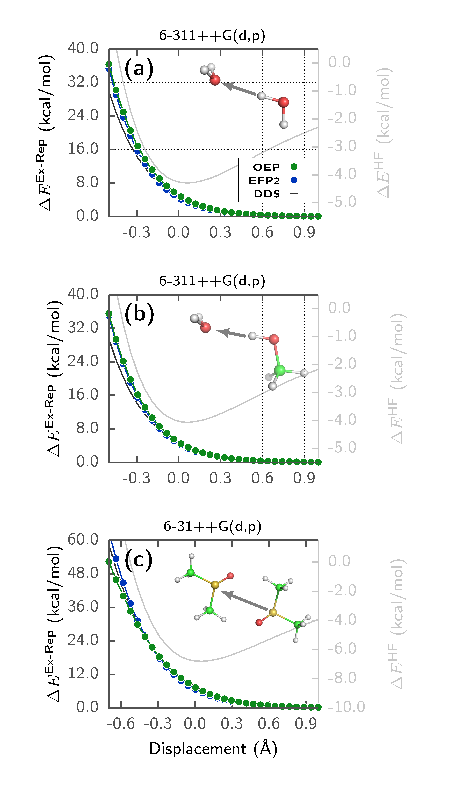
\includegraphics[width=0.5\textwidth]{fig-1.eps}
\caption{\label{f:fig-1} {\bf Performance of the DMS tensors of the ground\hyp{}state water molecule
in uniform electric field.} 
$R_{\rm max}$ denotes the maximum rank of the electric field
in the expansion from Eq.~\eqref{e:final-model.General}.
Electric field magnitudes in a range from 0.0 to 0.07 a.u. were tested in 100 samples with randomly selected 
directions of electric field.
} 
\end{figure}
%

All the tested models that are linear with respect to the electric field,
i.e., from Eq.~\eqref{e:final-model.HF} (black solid squares in Figure~\ref{f:fig-1}) 
as well as truncated at linear susceptibilities $\mathbb{B}^{(1)}$ 
from Eqs.~\eqref{e:dD-Taylor} (blue solid circles) and \eqref{e:final-model.General} (blue open circles),
incorrectly reproduce the polarization energy.
Interestingly, the predicted values are in strong
correlation with the exact estimates and exhibit similar slope of $\sim$2.
Incorporation of the second\hyp{}order term
obtained either by numerical differentiation from Eq.~\eqref{e:B20} (red filled circles) 
or by using the generalized DMS model (red open circles)
dramatically reduces the errors
leading to quantitative accuracy in all tested field magnitudes 
with the best RMSE of 0.173 kcal/mol ($R^2=99.1\%$) for the generalized DMS model.
On the other hand, the
induced dipole and quadrupole moments are reproduced reasonably well by
using the first\hyp{}order DMS with $R^2$ coefficients being 
greater than 97\% in case of dipole moments and from 69\% up to 81\% in case of quadrupole moments.
This observation can be understood given the fact that the induced dipole
and quadrupole moment is approximately proportional to the external electric field, whereas the polarization
energy exhibits quadratic dependence (c.f. Eq.~\eqref{e:dE-dpol}), hence the need of including at least
quadratic terms in the expansion from Eq.~\eqref{e:dD-Taylor} or Eq.~\eqref{e:final-model.General}. 

In comparison to the dipole\hyp{}dipole polarizability approach, 
quadratic DMS models perform only slightly worse 
(for example, RMSE = 0.173 and 0.112 kcal/mol when the generalized quadratic DMS
model and the polarizability model are used, respectively).
However, quadratic DMS models better predict the induced multipole moments with
$R^2$ systematically greater than 99\%. 
Certainly, taking into account the distributed quadrupole polarizabilities
would greatly reduce errors of the standard distributed polarizability approach.
Nevertheless, it is clear that the second\hyp{}order
DMS models are quantitative even at very strong uniform electric fields.

%
\begin{table*}%[]
\caption[Performance of the DMS tensors of ground\hyp{}state water molecule
in uniform and non\hyp{}uniform electric field]{\label{t:results}
{\bf Performance of the DMS tensors of ground\hyp{}state water molecule
in uniform and non\hyp{}uniform electric field}  
\footnotemark[1]\footnotemark[2]
}
%\begin{ruledtabular}
\resizebox{\textwidth}{!}{%
\begin{tabular}{cddddddcddddcdd}
\hline\hline
%\toprule
\multicolumn{1}{l}{} & \multicolumn{6}{c}{\textbf{Ab Initio DMS}} &  & \multicolumn{4}{c}{\textbf{Generalized DMS}}
                                                                  &  & \multicolumn{2}{c}{\textbf{Distributed}} \\
\cline{2-8}
\cline{9-12}
%\cline{14-15}
\textbf{}         
& \multicolumn{2}{c}{$\BM{R_{\rm max}=1}$\footnotemark[3]}
& \multicolumn{2}{c}{$\BM{R_{\rm max}=1}$\footnotemark[4]}
& \multicolumn{2}{c}{$\BM{R_{\rm max}=2}$\footnotemark[4]}
&
& \multicolumn{2}{c}{$\BM{R_{\rm max}=1}$\footnotemark[5]} 
& \multicolumn{2}{c}{$\BM{R_{\rm max}=2}$\footnotemark[5]} 
&  
& \multicolumn{2}{c}{\textbf{Polarizability}}        \\ \hline
\multicolumn{15}{c}{} \\ 
\multicolumn{15}{c}{\textbf{Uniform Electric Field}} \\ 
\multicolumn{15}{c}{} \\ \hline
\multicolumn{1}{l}{} & \multicolumn{14}{c}{\textbf{RMSE (kcal/mol)}}              \\ %\hline
   & 4.041 & (n.d) & 4.823 & (n.d.) & 0.231 & (98.40) && 5.0121 & (n.d.) & 0.173 & (99.10) && 0.112 & (99.63) \\ 
\multicolumn{1}{l}{} & \multicolumn{14}{c}{\textbf{RMSD (mD)}}                    \\ %\hline
   & 30.46 & (97.91) & 30.46 & (97.91) & 18.02 & (99.27) && 24.83 & (98.61) & 7.13 & (99.89) && 30.46 & (97.91) \\ 
\multicolumn{1}{l}{} & \multicolumn{14}{c}{\textbf{RMSQ (D\AA $\times 10^{-3}$)}} \\ %\hline
   & 47.89 & (69.17) & 39.24 & (79.30) &  8.56 & (99.02) && 37.63 & (80.96) & 3.94 & (99.79) && 50.66 & (65.49) \\ \hline
\multicolumn{15}{c}{} \\ 
\multicolumn{15}{c}{\textbf{Non-Uniform Electric Field}\footnotemark[6]} \\ 
\multicolumn{15}{c}{} \\ \hline
\multicolumn{1}{l}{} & \multicolumn{14}{c}{\textbf{RMSE (kcal/mol)}}   \\ 
W & 0.067 & (n.d.)  & - &  -  & - &  -  && 0.076 & (n.d.)  & 0.003 & (99.45) && 0.004 & (98.64) \\ 
M & 1.072 & (n.d.)  & - &  -  & - &  -  && 1.236 & (n.d.)  & 0.057 & (99.08) && 0.070 & (98.58) \\ 
S & 4.220 & (n.d.)  & - &  -  & - &  -  && 5.147 & (n.d.)  & 0.402 & (97.25) && 0.332 & (98.13) \\ \hline
\multicolumn{1}{l}{} & \multicolumn{14}{c}{\textbf{RMSD (mD)}}  \\ 
W &  3.36 & (98.71) & - &  -  & - &  -  &&  1.03 & (99.88) &  0.94 & (99.90) &&  3.36 & (98.71) \\ 
M & 14.72 & (98.50) & - &  -  & - &  -  &&  7.72 & (99.59) &  4.55 & (99.86) && 14.72 & (98.50) \\ 
S & 44.80 & (96.92) & - &  -  & - &  -  && 33.06 & (98.33) & 15.96 & (99.61) && 44.80 & (96.92) \\ \hline
\multicolumn{1}{l}{} & \multicolumn{14}{c}{\textbf{RMSQ (D\AA $\times 10^{-3}$)}} \\ 
W &  6.22 & (58.72) & - &  -  & - &  -  &&  1.59 & (97.32) &  1.42 & (97.86) &&  5.45 & (68.29) \\ 
M & 28.22 & (53.90) & - &  -  & - &  -  && 10.45 & (93.68) &  5.68 & (98.13) && 23.94 & (66.83) \\ 
S & 78.07 & (40.53) & - &  -  & - &  -  && 43.33 & (81.68) & 14.40 & (97.98) && 64.33 & (59.62) \\ 
%\bottomrule
\hline\hline
\end{tabular}%
}
%\end{ruledtabular}
\footnotetext[1]{$R$-squared coefficients are shown in parentheses. `$n.d.$' stands for `not determined'.}
\footnotetext[2]{Ranks of the density matrix susceptibility models are denoted as $R_{\rm max}$ where $R_{\rm max}$ is the maximum power in the expansion from Eq.~\eqref{e:final-model.General}.}
\footnotetext[3]{\emph{Ab initio} HF model, Eq.~\eqref{e:final-model.HF}.}
\footnotetext[4]{\emph{Ab initio} finite\hyp{}difference model, Eq.~\eqref{e:dD-Taylor}.}
\footnotetext[5]{Linear\hyp{}regression generalized model, Eq.~\eqref{e:final-model.General}.}
\footnotetext[6]{`W', `M' and `S' denote `weak', `moderate' and `strong' electric fields that are generated by sets of point charges, respectively (c.f. Table~\ref{t:fields}).}
\end{table*}

\subsection{\label{ss:42}Water molecule in spatially non\hyp{}uniform electric field}

To study the capability of the distributed DMS models to capture 
density matrix polarization in inhomogeneous electric fields, a water molecule
surrounded by point charges is analyzed.
Three different types of point charge environment that generate
weak (0.003 -- 0.007 a.u.), 
moderate (0.01 -- 0.02 a.u.) and strong (0.02 -- 0.05 a.u.) 
electric fields around the water molecule were considered (Table~\ref{t:fields}),
%
\begin{table}[b]
\caption[Average electric fields in statistical sets of electrostatically perturbed ground states
of water molecule surrounded by point charges]
{{\bf Average electric fields in statistical sets of electrostatically perturbed ground states
of water molecule surrounded by point charges\footnotemark[1]}
}
\label{t:fields}
\begin{ruledtabular}
\begin{tabular}{ldcdcdcd}
\multirow{2}{*}{\textbf{Set\footnotemark[2]}} 
                                  & \multicolumn{7}{c}{\textbf{Average Electric Field (a.u.)}}      \\
                                  & \multicolumn{3}{c}{\textbf{Oxygen Atom}} & \textbf{} 
                                  & \multicolumn{3}{c}{\textbf{Hydrogen Atom}} \\
\cline{2-4}
\cline{6-8}
\textbf{W}                    & 0.0046     & $\pm$     & 0.0019     &           & 0.0046     & $\pm$     & 0.0020     \\
\textbf{M}                    & 0.0184     & $\pm$     & 0.0075     &           & 0.0186     & $\pm$     & 0.0078     \\
\textbf{S}                    & 0.0368     & $\pm$     & 0.0150     &           & 0.0372     & $\pm$     & 0.0156    
\end{tabular}
\end{ruledtabular}
%
\footnotetext[1]{Each set was composed of 100 samples differing in the configuration of 40 charges generated from a uniform distribution.}
\footnotetext[2]{`W', `M' and `S' denote `weak', `moderate' and `strong' electric fields, respectively.}
\end{table}
%
because similar ranges of electric field are experienced by water molecules
in liquid phase.\cite{Fried.Wang.Boxer.Ren.Pande.JPCB.2013,Reischl.Kofinger.Dellago.MolPhys.2009}
Performance descriptors of the \emph{ab initio} and generalized 
models of the density matrix susceptibility, as well as 
the conventional dipole\hyp{}dipole distributed polarizability
approach, are shown in Table~\ref{t:results}, whereas the error distributions
in strong electric fields are additionally plotted in Figure~\ref{f:fig-2}A--I.

Similarly as in uniform electric field, 
the \emph{ab initio} DMS model from Eq.~\eqref{e:final-model.HF} 
as well as the generalized linear DMS model, are insufficient to correctly describe the polarization energy 
in non\hyp{}uniform electric field, although the correlation with benchmark is still very clear with a slope of $\sim$2
(Figure~\ref{f:fig-2}A). Again, induced dipole moments are reproduced very well also
in strong electric fields (RMSD of 44.8~mD and lesser, $R^2>96\%$; Figure~\ref{f:fig-2}D and \ref{f:fig-2}E).
Induced quadrupole moments are well described only by the generalized DMS model.
For example, in moderate electric fields RMSQ is 10.4$\times 10^{-3}$D\AA{ }with $R^2=93.7\%$
whereas the \emph{ab initio} DMS model yields RMSQ of 28.2$\times 10^{-3}$D\AA{ }($R^2=53.9\%$).

\begin{figure*}[h]
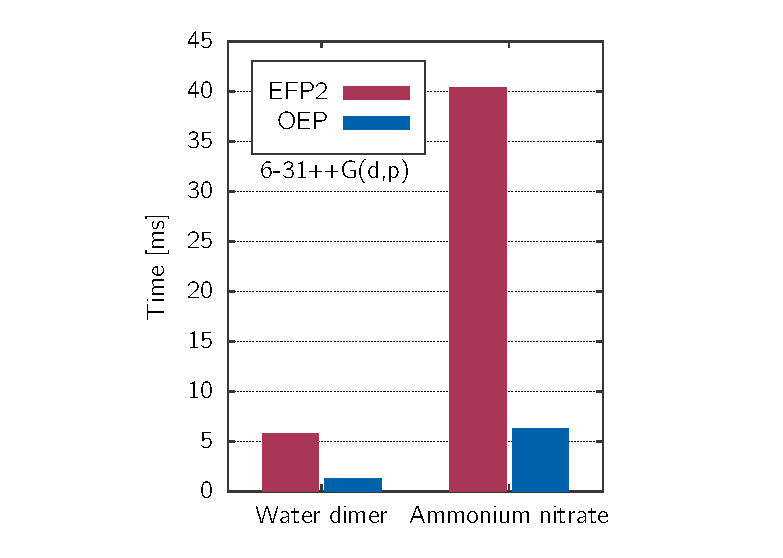
\includegraphics[width=\textwidth]{fig-2.eps}
\caption{\label{f:fig-2} {\bf Performance of the distributed DMS tensors of ground\hyp{}state water molecule in strong
non\hyp{}uniform electric field.}
In this Figure, `Ab Initio DMS' (panels A, D and G) 
refers to the model from Eq.~\eqref{e:final-model.HF} and
`Generalized DMS' (panels B, E and H) 
refers to the generalized model with $R_{\rm max}=2$ 
where $R_{\rm max}$ is the maximum power
in the expansion from Eq.~\eqref{e:final-model.General}.
Comparison with the distributed dipole\hyp{}dipole polarizability model %(Eq.~\eqref{e:dE-dpol})
is also shown in this Figure in panels C, F and I. 
The ensemble of electric fields corresponds to the `S' set
from Tables~\ref{t:results} and \ref{t:fields}.}
\end{figure*}

The most sophisticated model studied in this work, the generalized quadratic DMS model, yields excellent predictions 
of the polarization energies and induced multipole moments in all strengths of the non\hyp{}uniform electric field tested.
The errors in predicting polarization energy are reduced by over an order of magnitude when compared with
the linear DMS models. Improvement of accuracy can also be observed in the case of induced multipole moment predictions
but the effect is less significant.
%(improvement roughly by a factor of 2).
What is particularly interesting is that in weak and moderate electric fields
the generalized quadratic DMS model performs better than the distributed dipole\hyp{}dipole
polarizability model, whereas only in strong electric fields the situation is reversed
(RMSE of 0.402, $R^2=97.2\%$ and 0.332 kcal/mol, $R^2=98.1\%$ for the DMS and polarizability model, respectively; 
see also Figure~\ref{f:fig-2}B and \ref{f:fig-2}C).
Nevertheless, the quadratic DMS model yields still very accurate predictions 
of polarization energy and induced multipole moments, even in strong electric field.

Recently, it was found by Fried et~al. by performing molecular dynamics simulations with a classical 
polarizable force field, that the average electric field experienced by water molecule in liquid phase
in room temperature is around 0.014 a.u. ($\sim$70 MV/cm).\cite{Fried.Wang.Boxer.Ren.Pande.JPCB.2013}
This value corresponds to our moderate electric field set of samples (denoted as `M' in Tables~\ref{t:results}
and \ref{t:fields}) for which the
accuracy of the generalized quadratic DMS model is excellent.
Water molecules can experience
stronger electric fields in certain geometries of hydrogen bonded clusters, 
even up to 0.055 a.u. according to study by Reischl et~al.\cite{Reischl.Kofinger.Dellago.MolPhys.2009} 
This electric field magnitude falls into our strong electric field regime (denoted as `S')
in which the generalized quadratic DMS model still provides accurate predictions (see also error distributions 
in Figure~\ref{f:fig-2}B, \ref{f:fig-2}E and \ref{f:fig-2}H). Therefore, it is believed that
the generalized quadratic DMS model is capable of accurately describing 
the polarization of ground\hyp{}state water molecule in inhomogeneous 
electric fields that are comparable in strength to condensed phase conditions.

\subsection{\label{s:computational-cost}Computational cost and automatization of the generalized DMS model}

Although the cost of computation of the perturbed one\hyp{}electron density matrices
from the generalized DMS tensors and the distribution of the electric field is negligible, 
obtaining the generalized DMS tensors for a particular molecule
involves substantial amount of full QM calculations. %necessary to fit the DMS tensor elements.
This is, however, a relatively expensive operation that has to be performed only once
when the EFP\hyp{}like strategy is adopted. 
%Note that the DMS parameters 
%are environment\hyp{}independent and, due to this reason, could be used
%as effective fragment parameters.
%To get statistically relevant set of perturbed states, it is recommended to perform at least 100 
%full QM calculations. 
Note also that each of such preparatory calculations is an independent computational task, 
and hence, its automatization and parallelization is straightforward. Moreover, the implementation
of the method does not depend on the level of theory because only the perturbed density matrices
are needed. The least\hyp{}squares fit, i.e., the computation of the gradient
and Hessian matrix including its inversion, is inexpensive.
This step can be implemented in an independent script or program taking as input the
perturbed density matrices obtained by using any available quantum chemistry package. 
%and its efficiency is limited only by the speed of Hessian matrix inversion.
Therefore, the linear regression method to obtain the DMS tensors could be applied 
to any molecular fragment at a chosen level of theory
in a fairly black box manner, provided that
the one\hyp{}particle density matrices are available. In the illustrations shown in this work,
a set of 100 independent full QM calculations was sufficient to get statistically relevant set of perturbed 
ground state density matrices. 
%This task was concluded within approximately 5 minutes per each DMS fit
%on a single\hyp{}CPU computer.

\section{\label{s:5}Summary and a few concluding remarks}

In this work, it was demonstrated that the generalized DMS models from Eq.~\eqref{e:final-model.General}
can accurately describe the polarization\hyp{}induced deformation 
of the one\hyp{}particle ground\hyp{}state electronic density
due to the uniform and non\hyp{}uniform distribution of electric field.
It was also shown that the accuracy of the model can be improved 
by extending the parameter space of the susceptibility tensors.
Even at the current state of development, the generalized quadratic DMS model
is of comparable and quantitative energetic accuracy as the distributed 
polarizability model (RMSE of 0.4~kcal/mol in strong 
electric fields and less than 0.06~kcal/mol in moderate and weak fields).
Moreover, any type of one\hyp{}particle density matrix could be treated by using
generalized DMS models, which is much more difficult to realize when a conventional multipole
model is used. Therefore, it is believed that the generalized DMS approach
has an important advantage over the multipole\hyp{}based approach, i.e., it provides more detailed
tensor description of the spatial polarization of the electron density distribution, that could be
combined for example with density\hyp{}based methods of interaction energy calculations.\cite{Mandado.Hermida-Ramon.JCTC.2011}

It is anticipated here that the generalized models from Eq.~\eqref{e:final-model.General}
should be studied in the future with an emphasis 
on their further optimization and application for molecular aggregates.
For this purpose, more general forms of Eq.~\eqref{e:final-model.General}, 
as well as the choice of distributed
sites should be further investigated, preferably considering post\hyp{}Hartree\hyp{}Fock methods
and electronically excited states.
Nevertheless, owing to the capability of the proposed approach to correctly capture the 
polarization of ground state's electron density,
the generalized density matrix susceptibility tensors 
could be used in accurate fragment\hyp{}based calculations of extended molecular aggregates
described at correlated levels of theory, particularly including the excited state chemistry.

\begin{acknowledgments}
This project is carried out under POLONEZ programme which has received funding from the European Union's
Horizon~2020 research and innovation programme under the Marie Skłodowska-Curie grant agreement 
No.~665778. \InlineImage{eu-logo.eps} This project is funded by National Science Centre, Poland 
(registration No.~2016/23/P/ST4/01720) within the POLONEZ 3 fellowship. 
\end{acknowledgments}

%
\appendix

\section{\label{a:orig-dep} Origin-Independence of the Induced Dipole Moment}

Multipole one\hyp{}electron integrals depend on the origin with respect to which they are evaluated.
However, the induced dipole moment defined in Eq.~\eqref{e:L-projector} 
has to be origin\hyp{}independent. Denoting the overlap AO integrals 
by $S_{\alpha\beta} = \braket{\alpha}{\beta}$,
it follows that $\mathbb{M}_u({\bf r}_Q) = \mathbb{M}_u({\bf 0}) - u_Q {\bf S}$
for $u=x,y,z$. Thus,
%
\begin{equation}
 \mathbb{L}_u({\bf r}_Q) = \mathbb{L}_u({\bf 0})
                          - u_Q {\bf C}^{(0)\dagger} \cdot {\bf S} \cdot \left( {\bf 1} - {\bf D}^{(0)}\right) \;,
\end{equation}
%
where
%
\begin{equation}
 \mathbb{L}_u({\bf 0}) = {\bf C}^{(0)\dagger} \cdot \mathbb{M}_u({\bf 0}) \cdot \left( {\bf 1} - {\bf D}^{(0)}\right) \;.
\end{equation}
%
But
%
\begin{equation}
  {\bf C}^{(0)\dagger} \cdot {\bf S} \cdot \left( {\bf 1} - {\bf D}^{(0)}\right) 
= {\bf C}^{(0)\dagger} \cdot \left( {\bf S} - {\bf 1} \right)
\end{equation}
%
since ${\bf C}^{(0)\dagger} \cdot {\bf S} \cdot {\bf C}^{(0)} = {\bf 1}$. 
In the simplest case of ${\bf S} = {\bf 1}$ (i.e., the AO basis functions are orthogonal) 
$\mathbb{L}_u({\bf r}_Q) = \mathbb{L}_u({\bf 0})$ which guarantees charge conservation.
When a non\hyp{}orthogonal AO basis is used, 
the following general condition must be satisfied:
%
\begin{equation}
 \Re \left\{
  \Tr{
  \left[
  \delta {\bf C} \cdot {\bf C}^{(0)\dagger} \cdot \left( {\bf S} - {\bf 1} \right)  
 \right]}
 \right\} = 0 \;.
\end{equation}
%
Due to the fact that ${\BM \Delta}$ considered here is accurate only up to first\hyp{}order, 
the above expression is not valid. 
Therefore, the polarization\hyp{}induced distributed dipole moments 
defined in Eq.~\eqref{e:L-projector} are exactly origin\hyp{}independent
as long as the AO basis is orthogonalized.
In such a case, one can compute one\hyp{}electron dipole integrals with respect to any origin 
and the resulting susceptibilities $\mathbb{B}^{(i;1)}$ 
from Eq.~\eqref{e:susceptibility-B} will be uniquely defined. They can be back\hyp{}transformed
to the original (non\hyp{}orthogonal) AO basis, 
${\bf X} \cdot \mathbb{B}^{(i;1)} \cdot {\bf X}$, where $\bf X$ is an orthogonalizer.
The numerical tests confirmed that $\Tr\left[\delta{\bf D}\cdot{\bf S}\right] \sim 10^{-16}$
with $\delta{\bf D}$ given by Eq.~\eqref{e:final-model.HF} and susceptibilities transformed
to the non\hyp{}orthogonal AO basis.

\section{\label{a:blocks} Explicit Formulae for Gradient and Hessian Blocks in Linear Regression DMS Model}

The gradient vector ${\bf g}$ and the Hessian matrix ${\bf H}$ 
are built from blocks associated with a particular type of parameters, i.e.,
%
\begin{equation}\label{e:Newton.gH}
 {\bf g} = 
\begin{pmatrix}
{\bf g}^{[1]} \\ 
{\bf g}^{[2]} 
\end{pmatrix} ,\quad
 {\bf H} = 
\begin{pmatrix}
{\bf H}^{[11]} & {\bf H}^{[12]}  \\ 
{\bf H}^{[21]} & {\bf H}^{[22]}  
\end{pmatrix} \;,
\end{equation}
%
where the block indices 1 and 2 correspond to the first\hyp{} and second\hyp{}order susceptibilities, respectively.
Note that the second derivatives of $\delta D^{(N)}$ 
with respect to the adjustable parameters vanish
due to the linear functional form of Eq.~\eqref{e:final-model.General.Parameters}.
Thus, the gradient element of the $r$th block and Hessian element of the $(rs)$th block read
%
\begin{subequations}
 \begin{align}
  g^{[r ]}    &\equiv \frac{\partial   Z}{\partial s^{[r]}} 
     =-2\sum_N \overline{\delta D}^{(N)}
               \frac{\partial   \left[ \delta D^{(N)} \right]}{\partial s^{[r]}} \;,\\
  H^{[rs]} &\equiv \frac{\partial^2 Z}{\partial s^{[r]} \partial s^{[s]}}  
     = 2\sum_N 
        \frac{\partial   \left[ \delta D^{(N)} \right]}{\partial s^{[r]}}
        \frac{\partial   \left[ \delta D^{(N)} \right]}{\partial s^{[s]}} \;.
 \end{align}
\end{subequations}
%
The explicit formulae for the gradient are
%
\begin{subequations}
 \begin{align}
  g^{[1]}_{ku} &=-2\sum_N \overline{\delta D}^{(N)} F^{(N)}_{ku} \;,\\
  g^{[2]}_{kuw} &=-2r_{uw} \sum_N \overline{\delta D}^{(N)} F^{(N)}_{ku} F^{(N)}_{kw} \;.
 \end{align}
\end{subequations}
%
The Hessian subsequently follows to be
%
\begin{subequations}
 \begin{align}
  H^{[11]}_{ku,lw} &= 2\sum_N F^{(N)}_{ku} F^{(N)}_{lw} \;,\\
  H^{[12]}_{ku,lu'w'} &= 2r_{u'w'} \sum_N F^{(N)}_{ku} F^{(N)}_{lu'} F^{(N)}_{lw'}  \;,\\
  H^{[22]}_{kuw,lu'w'} &= 2r_{uw} r_{u'w'} \sum_N F^{(N)}_{ku} F^{(N)}_{kw} F^{(N)}_{lu'} F^{(N)}_{lw'} \;.
 \end{align}
\end{subequations}
%
Note that due to the symmetry of the Hessian matrix, the block $21$
is a transpose of the block $12$. The composite indices $ku$ and $kuw$ 
are constructed from the distributed site index $k$ and the appropriate 
symmetry\hyp{}adapted ($w<u$) Cartesian component of a particular DMS tensor: 
$u$ for the first\hyp{}order, and $uw$ for the second\hyp{}order susceptibility 
tensor, respectively. The method described above can be easily extended 
to third and higher orders.

% -----------------------
%\bibliographystyle{aipnum4-1}
\bibliography{references}
% -----------------------

\end{document}
